\subsection{Marenostrum}

\begin{frame}
\frametitle{Barcelona Supercomputing Center (BSC)}
	\begin{columns}
	\begin{column}{0.4\textwidth}
		\begin{itemize}
			\item \textit{Origin} by Dawn Brown, sci-fi
			\item 2005
			\item Public research center
			\item 60\% Spanish Governance
			\item 30\% Catalan Governance
			\item 10\% UPC Governance
			\item Money similar + industrial and european fundings
			\item \textbf{Host the most beautiful SuperComputer of the world}
		\end{itemize}
	\end{column}
	\begin{column}{0.6\textwidth}
		\begin{figure}[H]
			\centering
			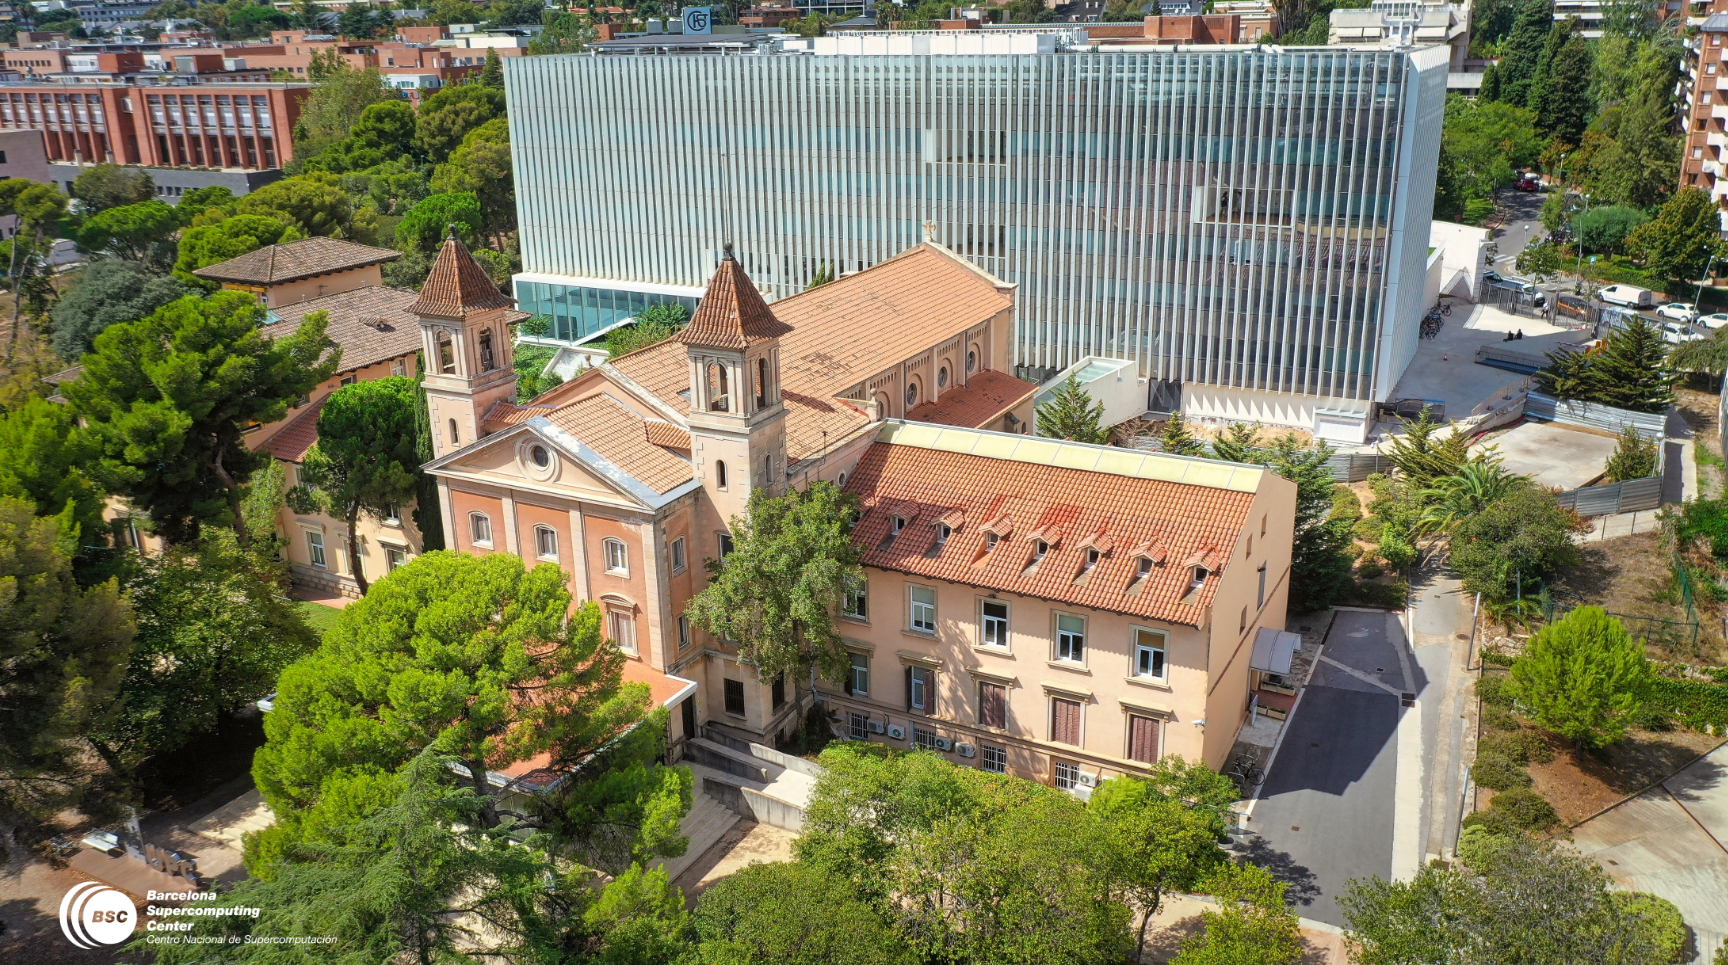
\includegraphics[width=\textwidth]{church_and_repsol.png}
			\caption{The deconsecrated church and Repsol.}
		\end{figure}
	\end{column}
	\end{columns}
\end{frame}


\begin{frame}
	\only<1>{
		\frametitle{Marenostrum 1}
		\begin{columns}
		\begin{column}{0.4\textwidth}
			\begin{itemize}
				\item 2004
				\item IBM and Spanish gov. sign contract
				\item 42.35 TeraFlop/s
			\end{itemize}
		\end{column}
		\begin{column}{0.6\textwidth}
			\begin{figure}[H]
				\centering
				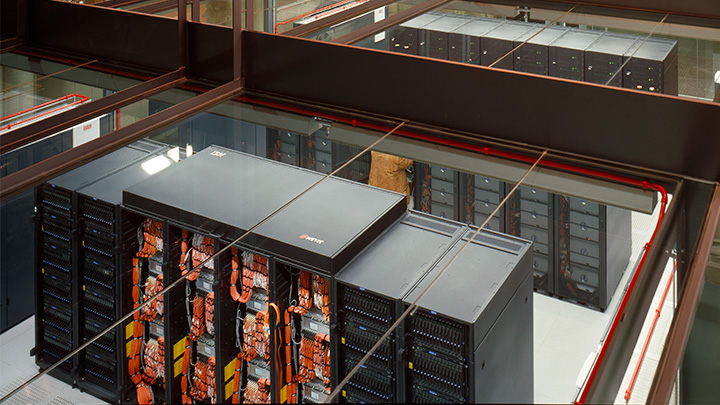
\includegraphics[width=\textwidth]{mn1.jpg}
				\caption{Marenostrum 1.}
			\end{figure}
		\end{column}
		\end{columns}
	}
	\only<2>{
		\frametitle{Marenostrum 2}
		\begin{columns}
		\begin{column}{0.4\textwidth}
			\begin{itemize}
				\item 2006
				\item extension of MN1
				\item 2x the Perf.
				\item 4812 cores to 10240
				\item 94.21 TeraFlop/s
			\end{itemize}
		\end{column}
		\begin{column}{0.6\textwidth}
			\begin{figure}[H]
				\centering
				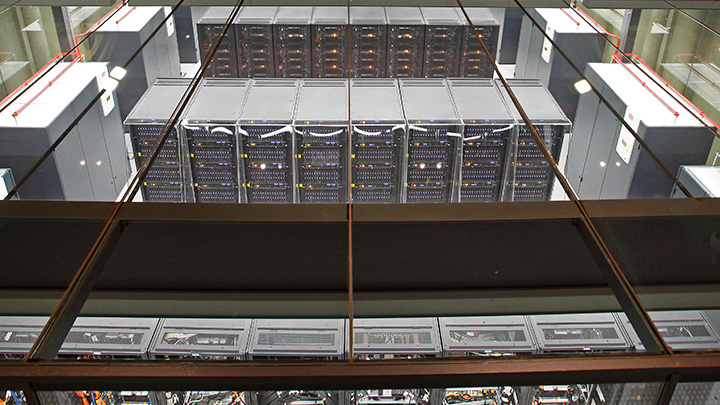
\includegraphics[width=\textwidth]{mn2.jpg}
				\caption{Marenostrum 2.}
			\end{figure}
		\end{column}
		\end{columns}
	}
	\only<3>{
		\frametitle{Marenostrum 3}
		\begin{columns}
		\begin{column}{0.4\textwidth}
			\begin{itemize}
				\item 2012
				\item 48896 cores of sandy bridge
				\item 1.1 PetaFlop/s
				\item 115 TeraByte of RAM
			\end{itemize}
		\end{column}
		\begin{column}{0.6\textwidth}
			\begin{figure}[H]
				\centering
				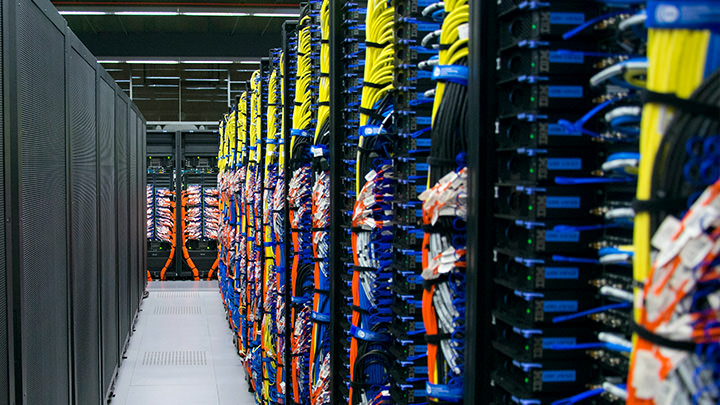
\includegraphics[width=\textwidth]{mn3.jpg}
				\caption{Marenostrum 3.}
			\end{figure}
		\end{column}
		\end{columns}
	}
	\only<4>{
		\frametitle{Marenostrum 4}
		\begin{columns}
		\begin{column}{0.4\textwidth}
			\begin{itemize}
				\item 2017
				\item 3456 nodes
				\item each node = 2 Intel Xeon with 24 cores
				\item 165888 processors
				\item 390 TeraBytes of RAM
				\item peak 13-ish PetaFlop/s
				\item 1.3 MegaWatt$\cdot$year
				\item Heterogeneous:
				\begin{itemize}
					\item MN4 CTE-Power
					\item MN4 CTE-AMD
					\item MN4 CTE-ARM
				\end{itemize}
			\end{itemize}
		\end{column}
		\begin{column}{0.6\textwidth}
			\begin{figure}[H]
				\centering
				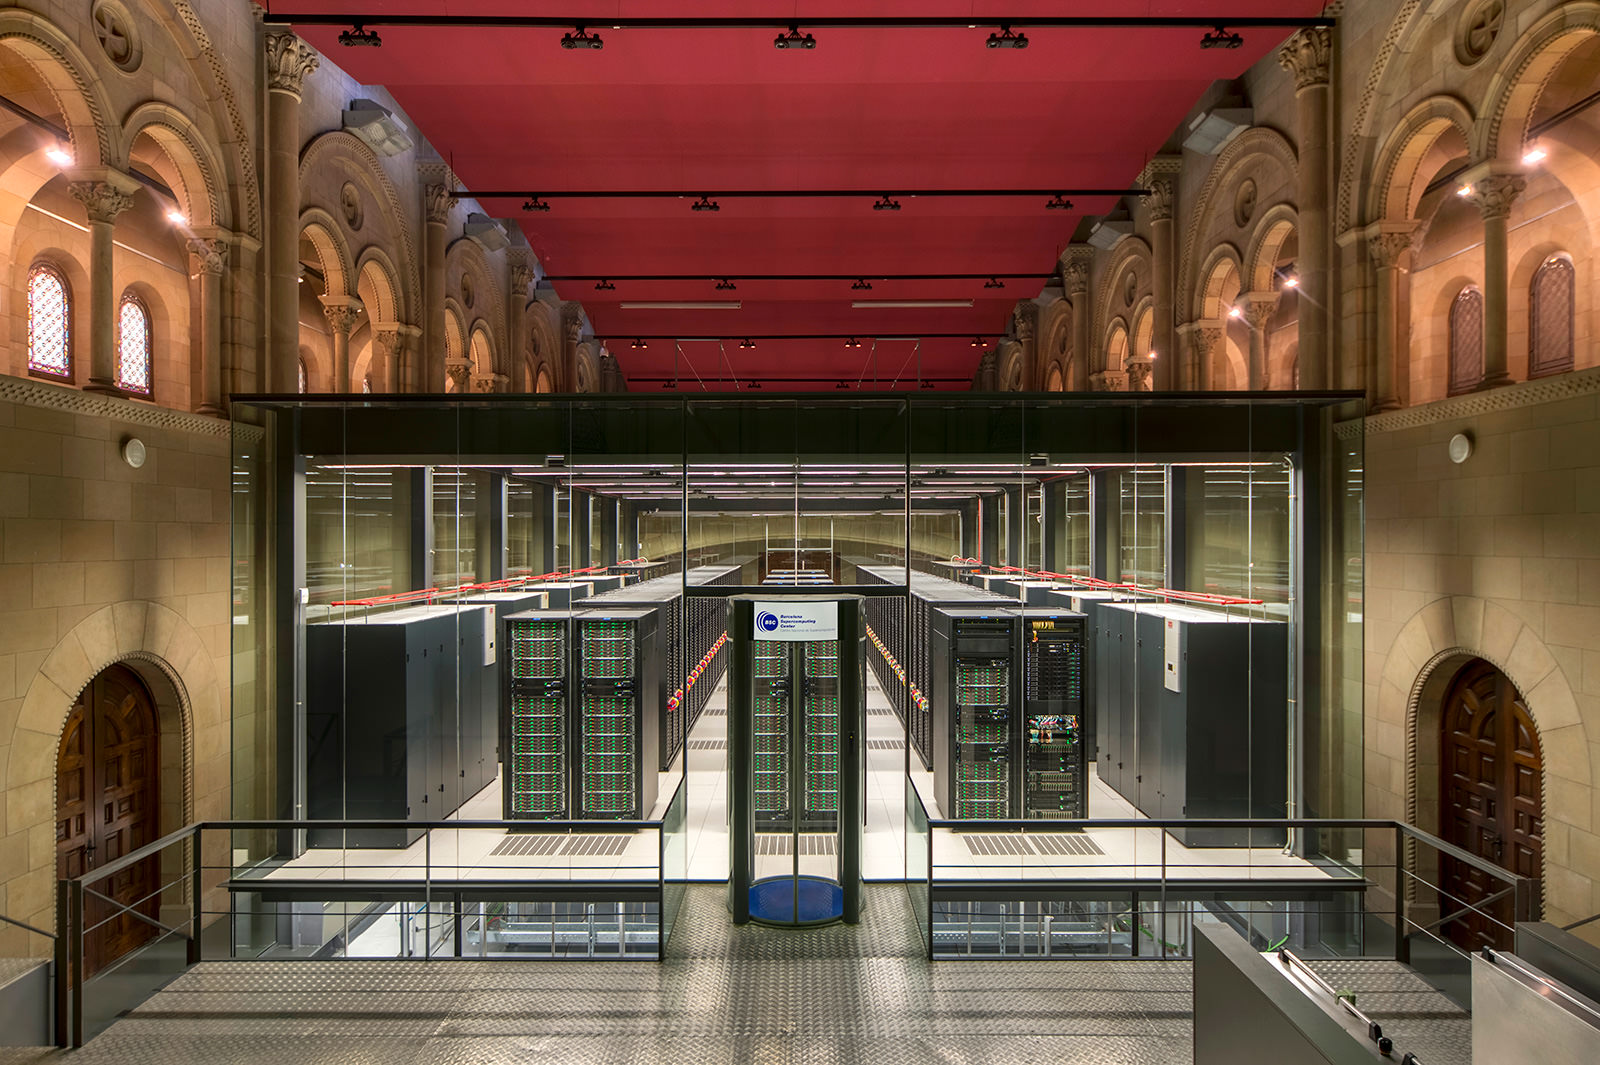
\includegraphics[width=\textwidth]{mn4.jpg}
				\caption{Marenostrum 4.}
			\end{figure}
		\end{column}
		\end{columns}
	}
	\only<5>{
		\frametitle{Marenostrum 5}
		\begin{columns}
		\begin{column}{0.4\textwidth}
			\begin{itemize}
				\item 2020 (2023 really)
				\item top500 now: 11th (acc) and 35th (gpp)
				\item top500 october: top8
				\item \textit{pre-exascale} 175 PetaFlop/s
				\item 10MW$\cdot$year
				\item \textbf{No more the most beautiful SC of the world, RIP :')}
				\item one node of MN5 is the full church of MN1
			\end{itemize}
		\end{column}
		\begin{column}{0.6\textwidth}
			\begin{figure}[H]
				\centering
				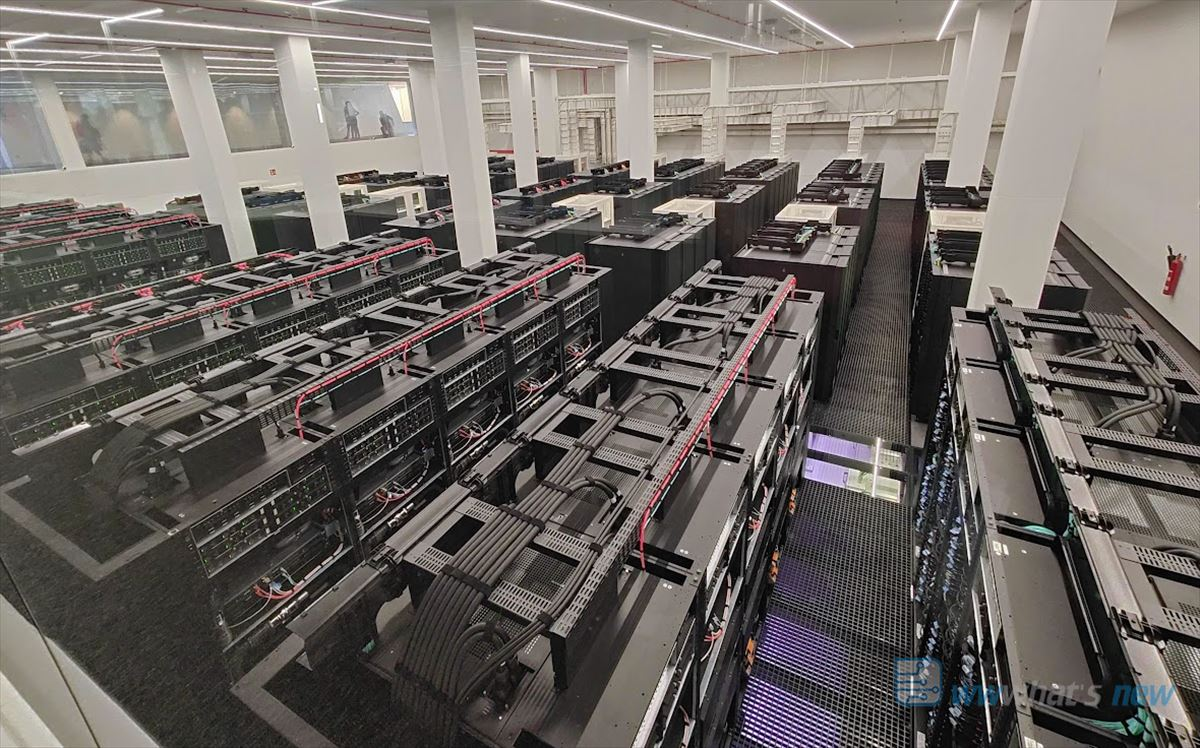
\includegraphics[width=\textwidth]{mn5.jpg}
				\caption{Marenostrum 5.}
			\end{figure}
		\end{column}
		\end{columns}
	}
\end{frame}
